\section{Background}

The eduROV project started as an idea at Trondheim Maker Faire in 2014. From there on it has been developed into a \emph{"functioning Open-Source ROV project at a new level of affordability."} \citep{edurov}. The project is managed by Norwegian University of Science and Technology (NTNU) and in specific the \emph{engage} project by Centre for Engaged Education through Entrepreneurship. It aims to let hobbyists, enthusiasts and schools to create a simple, affordable and open-source underwater ROV. From the 25th of June until July the 6th a summer school will be hosted at NTNU where high school student will build and test this ROV.

I, the author of this thesis, had participated in a course where I developed a similar ROV. In Desember 2017 I joined the project to improve the software which was used to control and display information from the ROV. There was three main areas that needed software improvements. First, the video latency was almost 800ms when using a cabled ethernet connection. Secondly, the software provided little to none user customization. Lastly, the user interface was not very attractive and had few features.

The ROV consisted of a Raspberry Pi 3 Model B+ (RPi) and an Arduino Micro. The Arduino was responsible for reading sensor values and controlling motors. The RPi had multiple tasks, it communicated with the Arduino by reading sensor values and sending motor speed commands. In addition, it captured video from the RPi camera module and displayed this to the user. Lastly, it processed user input from the operator and forwarded these commands to the Arduino.

On the RPi a python program using the \emph{Pygame} package was running. This is an open source package created for making games, but it can also be used to display video feed and read user input. When initiated, this program would display a window on the RPi. \emph{RealVNC}, a software for remote desktop viewing was then used to display this window on the remote computer used for control. \figref{edurovOld} shows this user interface (UI). The software did not require any installation, instead the correct files had to be copied from a GitHub repository.

\begin{figure}[h!]
    \centering
    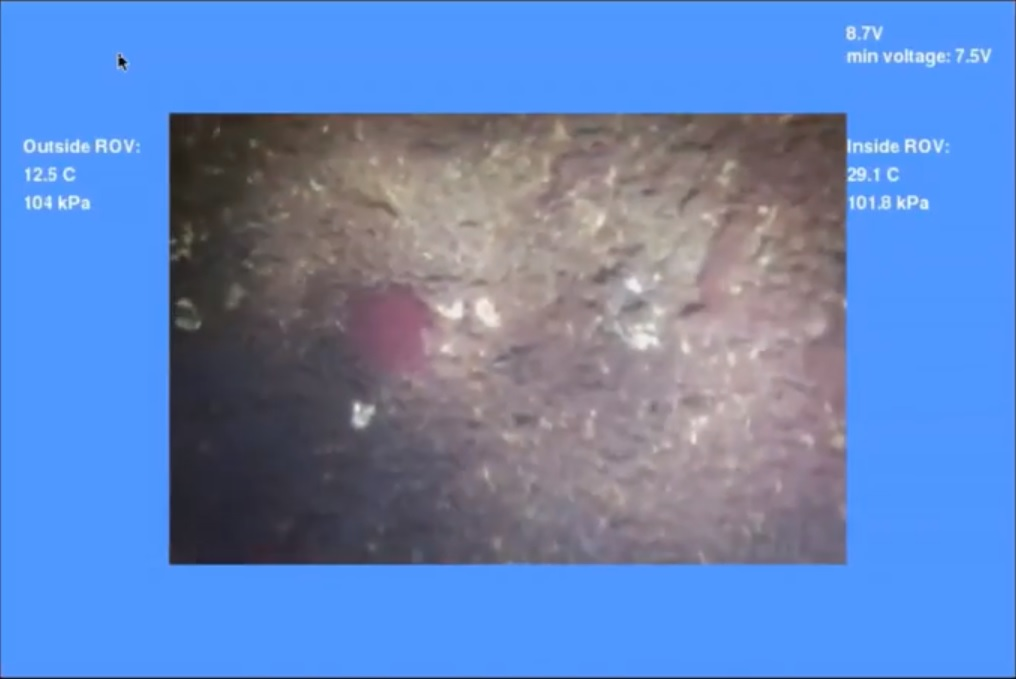
\includegraphics[width=0.8\textwidth]{edurovOld}
    \caption{User interface for the original eduROV.}
    \label{edurovOld}
\end{figure}

Some goals were then set for my contribution to the project:

\begin{itemize}
\item Reduce the video latency as much as possible while still having the possibility for high resolution images.

\item Streamline the installation process, i.e. remove the need for visiting any website or manually coping files.

\item Remove the need for any third party applications, that would mean removing the RealVNC dependency for video transfer.

\item Increase customization while still maintaining a high level application programming interface (API).

\item Make the UI more attractive, include more UI features without overwhelming the operator.
\end{itemize}

\section{Current alternatives}

There exists a wealth of software's created for operating ROV's. This discussion will be limited to those that are open source and created in Python. The most well known and probably most used is the \emph{Robot Operating System} (ROS) which is ported to python as a client library called \emph{rospy}. Although a powerful framework, it does not not suit the needs of this project. Originally written C++, ROS was originally not created for python. This means that the documentation is mostly in C++ and for anyone who wanted to customize the eduROV software in the future would have learn ROS in addition to python. It was decided that making ROS fit the needs of the eduROV would require more time and be limiting to the development, in comparison to creating a tailored software from scratch.

There is also something called \emph{GoPiGo}. This started as a Kickstarter project and is now a hardware / software project that you can buy online. It provides robot communication with video feed, but the software seems to created specifically for the robots they sell. The software is also not created as a package meant for other users to build on.

In summary, there wasn't really any good software alternatives for the eduROV project. Actually, I was not able to find any python packages created for ROV communication with video support built in. There are many guides on the internet that will walk you through how to create this, but the whole process can be really intimidating for people with limited experience. In addition, many of the guides online require you to install multiple software's and download files from additional places. Not very user friendly. Also, in the guides online they often control ROV's by pushing buttons on a screen, not by keyboard input. Lastly, they contain limited to none documentation.

\section{Development}

\todo[inline]{
- Git with issues

- Branches

- PyPi and versioning scheme

- Python Package Index PyPi
}

\section{Architecture}
\todo[inline]{
- socket protocols / Pyro4

- HTTP Webserver, ethernet and wifi

- different processes / Parallelism

- camera capture
}

\missingfigure{Graphics showing the architecture, hardware and software}

\section{Graphical user interface}
\todo[inline]{
- html and js

- customizable

- in the context of engage

- attitude
}

\citep{Chen2007} "Attitude (i.e., pitch and roll) of a robotic vehicle may be easy to reference when there are other familiar objects (e.g., horizon, buildings, trees, etc.) in the re- mote environment.However, if those reference points are absent and the on-board cameras are fixed, operators sometimes find it surprisingly hard to accurately assess the attitude of their robotic vehicles."

\citep{Wang2004} Gravity-Referenced Attitude Display for Teleoperation of Mobile Robots

\citep{Chen2007} "The ideal view depends on the task; overall awareness and pattern recognition are optimized by exocentric views whereas the immediate environment is often viewed better egocentrically."
"overlaying information on video feed can potentially lead to cognitive tunneling"

\missingfigure{Image showing the GUI of the eduROV submersible}

\section{Application programming interface}

\todo[inline]{
- WebMethod
}

\section{Performance}

\missingfigure{Image showing the video latencies at different resolutions}

\section{Documentation}

\todo[inline]{
- Read the docs with git

- Restructured text

- Autodoc with git

- Examples
}

\missingfigure{example code of how the documentation is written}

\missingfigure{example image of how this text is shown in the web browser}

\section{Novelty features}

\todo[inline]{
- main features from docs

- what does it do better than the competition

- future work

- websockets

- flask?
}